\documentclass[es,practica,12pt]{uah}

\tema{5}
\titulo{Códigos de paridad}{Lesson title}
%
\begin{document}

\titulacion{Optativa GIEC y GIT}
\departamento{Teoría de la Señal y Comunicaciones}
\asignatura{Comunicaciones Digitales}{}
\curso{2021/2022}

\maketitle

\begin{abstract}
	Continuamos estudiando los códigos de canal con un segundo ejemplo: los códigos de paridad
\end{abstract}

\section{Introducción}

Los códigos de paridad representan otro ejemplo de códigos muy simples para la detección de errores. En este caso, dada una palabra de $n-1$ bits, se añade un bit extra (bit de paridad) de forma que el número total de ``unos'' en la palabra código final sea par (paridad par)
 o impar (paridad impar). Su principal ventaja es la simplicidad, aunque tienen la desventaja de que sólo permiten detectar un número impar de errores y que no son capaces de corregirlos. Se utilizan habitualmente en aplicaciones hardware donde se puede repetir una operación en caso de encontrar algún error. Los buses PCI o SCSI utilizan este tipo de códigos.
 
 Otra aplicación interesante es en los sistemas RAID de discos duros. En este caso, si uno de los discos falla, se puede reconstruir la información combinando la información de los otros discos. Si tenemos, por ejemplo, un sistema RAID-5 con tres discos duros en el que los dos primeros tienen la siguiente información: ``\texttt{01010101}'' y ``\texttt{10001001}'' respectivamente, la información del tercer disco se calcula siguiendo un esquema de paridad, de forma que quedaría: ``\texttt{11011100}''. Si ahora falla cualquiera de los discos, su información se puede rescatar realizando la misma operación con los datos de los otros dos, tal y como se muestra en la siguiente figura:

 {\begin{figure*}[h!]\centering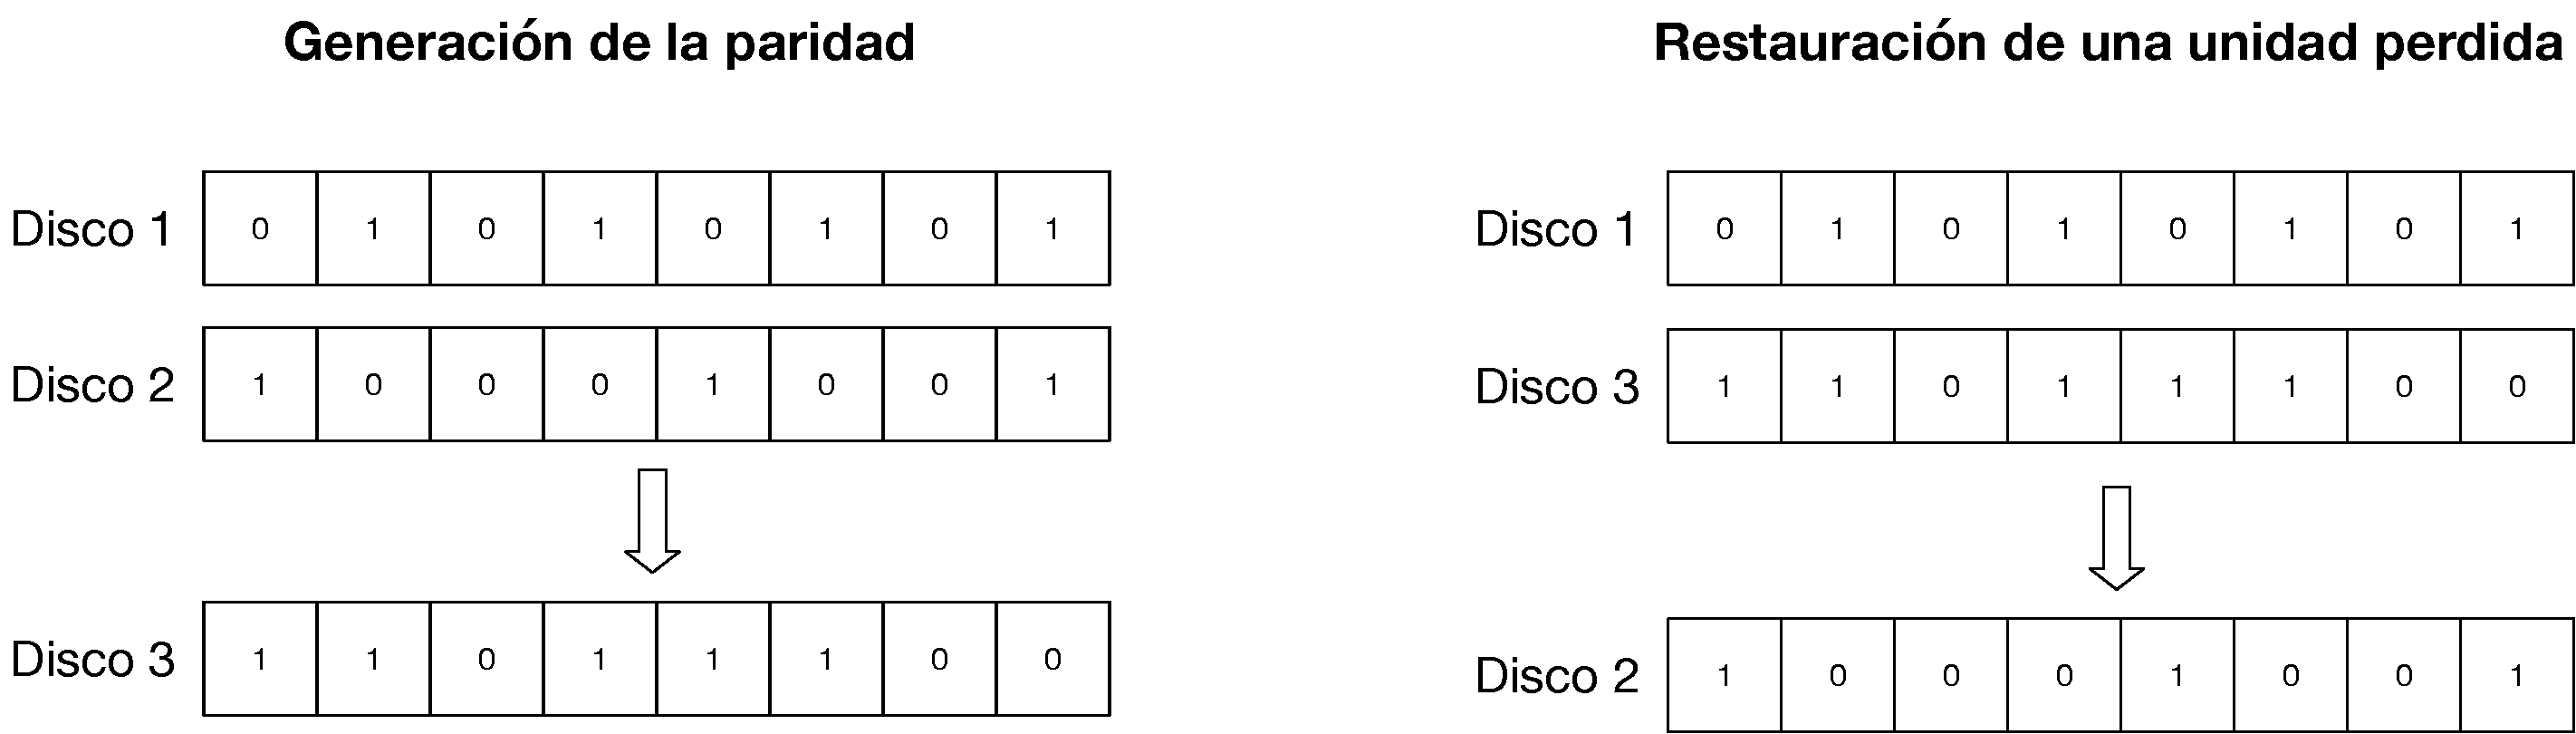
\includegraphics[width=14cm]{../Apuntes/Figuras/ParidadRAID}\end{figure*}


\section{Desarrollo de la práctica}


	\begin{enumerate}
		\item Generaremos en primer lugar una función en Matlab que, dado un array de dimensiones $1 \times N$ con bits para transmitir, genere un array $1 \times (N \frac{n}{n-1})$ con las palabras código obtenidas al utilizar un código de paridad par con palabras de $n$ bits, siendo el último el de paridad.
	
			La función debe tener el siguiente encabezado:
			
			\CodigoFuente{function codigo = CodificadorParidad(bits, n)}
	
		\item A continuación generaremos la función correspondiente al decodificador, que dado un vector $1 \times (N \frac{n}{n-1})$, compruebe cada una de las palabras código y marque aquellas en las que se haya detectado algún error, devolviendo un vector $1 \times N$.
		
			\CodigoFuente{function bits = DecodificadorParidad(codigo, n)}
				
		\item Para probar el sistema construido, vamos a volver a utilizar un vector con 10.000 bits aleatorios, que haremos pasar por el codificador, canal y decodificador configurados con $n=3$ y $p=0.02$:
		
			 \CodigoFuente{bitsTx = randi([0,1],[1,1e4]);}\\
			\CodigoFuente{codigoTx = CodificadorParidad(bitsTx, 3);}\\
			\CodigoFuente{codigoRx = Canal(codigoTx, 0.02);}\\
			\CodigoFuente{bitsRx = DecodificadorParidad(codigoRx, 3);}
		
			¿Cuál es la probabilidad de que no se haya detectado algún error?
		
	\end{enumerate}



\section{¿Qué entregar?}
\begin{itemize}
	\item Todas las funciones creadas.
	\item Script del ejemplo de Matlab (códigos de paridad).
\end{itemize}


%\printindex
\end{document}



	
